\chapter{提案手法}\label{method.tex}

\section{概要}

本章では, 空中署名による個人認証のための提案手法を述べる. 本研究における提案手法は図\ref{fig:ProposedMethod}に示すように3つのステップから構成される.
\\
\begin{figure}[htbp]
  \begin{center}
    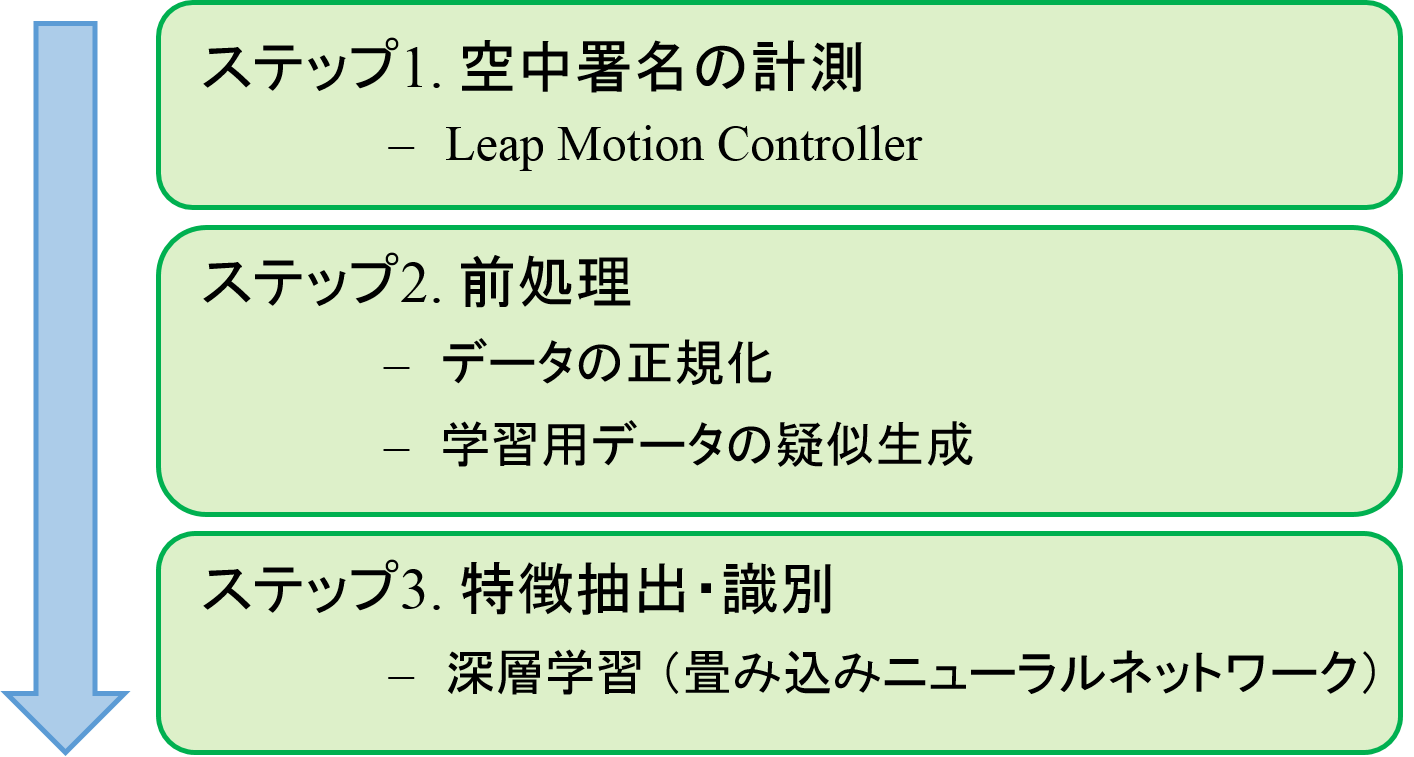
\includegraphics[clip,width=15.0cm]{./images/ProposedMethod.png}
    \caption{提案手法の流れ}
    \label{fig:ProposedMethod}
  \end{center}
\end{figure}\\

署名の計測にはLeap Motion Controllerを使用する. そして計測した署名データに対し前処理を行い, データを正規化する. 署名からの特徴抽出と識別には畳み込みニューラルネットワークによる深層学習を行う. ここで, 深層学習は機械学習手法の1つであり多くの学習用データが必要になる. しかし偽筆の学習用データを大量に用意するのは現実的には困難であると考えられるため, 前処理の段階で少量の学習用偽筆データに変形を加えることにより必要な学習用偽筆データを疑似生成する. 以下に各処理の詳細について述べる.\\

\section{空中署名の計測}

空中署名の計測にはLeap Motion Controllerを使用する. Leap Motion Controllerは2012年にLeap Motion社によって開発された小型USB周辺装置であり, 以下のような特徴がある.
\\
\begin{itemize}
  \item{手や指の動きを計測し, それらの3次元空間座標を計測する}
  \item{計測の精度は最大で0.01mm}
  \item{モニタやマウスには非接触}
  \item{追加の加速度センサやペンを身に付ける必要はない}\\
\end{itemize}

上記のように, Leap Motion Controllerは空中署名の計測機器として望ましい要素を備えており, 署名計測の正確性と利便性の向上に大いに役立つと考えられる. 図\ref{fig:LeapMotion}にLeap Motion Controllerの外観を示す.
\\
\begin{figure}[htbp]
  \begin{center}
    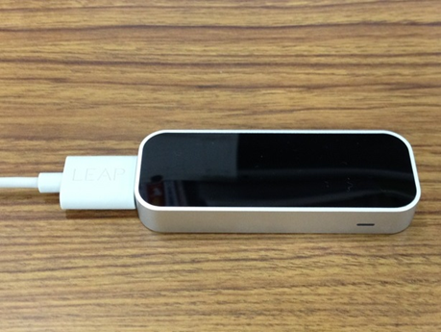
\includegraphics[clip,width=8.0cm]{./images/LeapMotion.png}
    \caption{Leap Motion Controllerの外観}
    \label{fig:LeapMotion}
  \end{center}
\end{figure}\\

装置上部の黒色の部分がセンサ面となり, 2基の赤外線センサと赤外線照射LEDが組み込まれている. センサ面の上部に存在する手や指が計測の対象となり, 得られる座標値は図\ref{fig:LeapAxes}のような直行直線座標系に基づく.本研究ではLeap Motion社から提供されているSDKを使用して制御を行う. 図\ref{fig:Demo}に空中署名の計測イメージを, 図\ref{fig:DemoKonishi}に実際に計測された署名データの例を示す. 

\begin{figure}[htbp]
  \begin{center}
    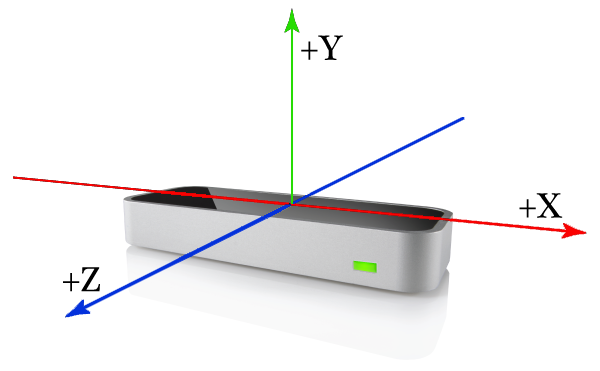
\includegraphics[clip,width=8.0cm]{./images/LeapAxes.png}
    \caption{Leap Motion Controllerの座標系(注1)}
    \label{fig:LeapAxes}
  \end{center}
\end{figure}

\begin{figure}[htbp]
  \begin{center}
    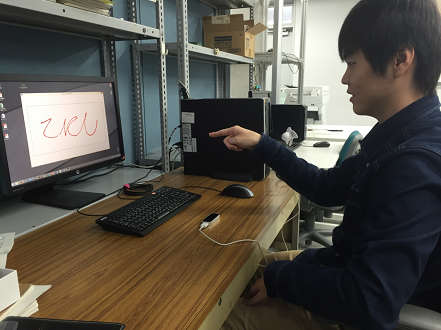
\includegraphics[clip,width=8.0cm]{./images/Demo.png}
    \caption{空中署名計測のイメージ}
    \label{fig:Demo}
  \end{center}
\end{figure}

\begin{figure}[htbp]
  \begin{center}
    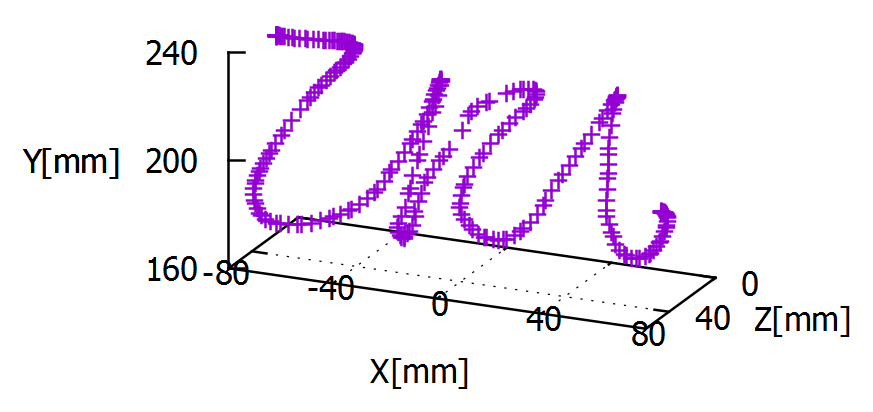
\includegraphics[clip,width=8.0cm]{./images/DemoKonishi.png}
    \caption{計測された空中署名の例}
    \label{fig:DemoKonishi}
  \end{center}
\end{figure}

\newpage

ここで, 電子タブレットであれば筆圧により文字間の運筆部分を容易に検出可能である. 一方, 筆圧の概念を持たない空中署名においては運筆部分の検出が非常に困難となる. しかしながら, 個人認証という側面から考えるに文字の区切りは必ずしも重要ではなく, 署名時の指先の軌跡全体を一連の署名動作と捉えることも可能である. そこで, 本研究では署名中の文字の分割等は行わずに図\ref{fig:DemoKonishi}のような一筆書きの署名として扱う. すなわち, 署名の開始から終了まで, 運筆部分を含めた指先の軌跡全てにおいて個人の癖や特徴が含まれていると仮定する.\\
\\
(注1) https://developer.leapmotion.com/documentation/cpp/devguide/Leap\_Overview.htmlより引用

\newpage

\section{前処理}

本研究では計測した署名を図\ref{fig:DemoKonishi}のように文字として扱うのではなく, 図\ref{fig:PreProcessing1}のようにXYZの3軸方向の座標に分解し, それぞれの1次元データとして扱う. これは, 各軸に対する指先の動きを捉えるためである. これらのデータに対し, 以下に述べる
\\
\begin{enumerate}
  \item 署名開始前・終了後の区間の削除
  \item 座標情報から動き情報への変換
  \item データ長の統一
  \item データ値のスケーリング\\
\end{enumerate}
の各処理を順次適用する.
\\
\begin{figure}[htbp]
  \begin{center}
    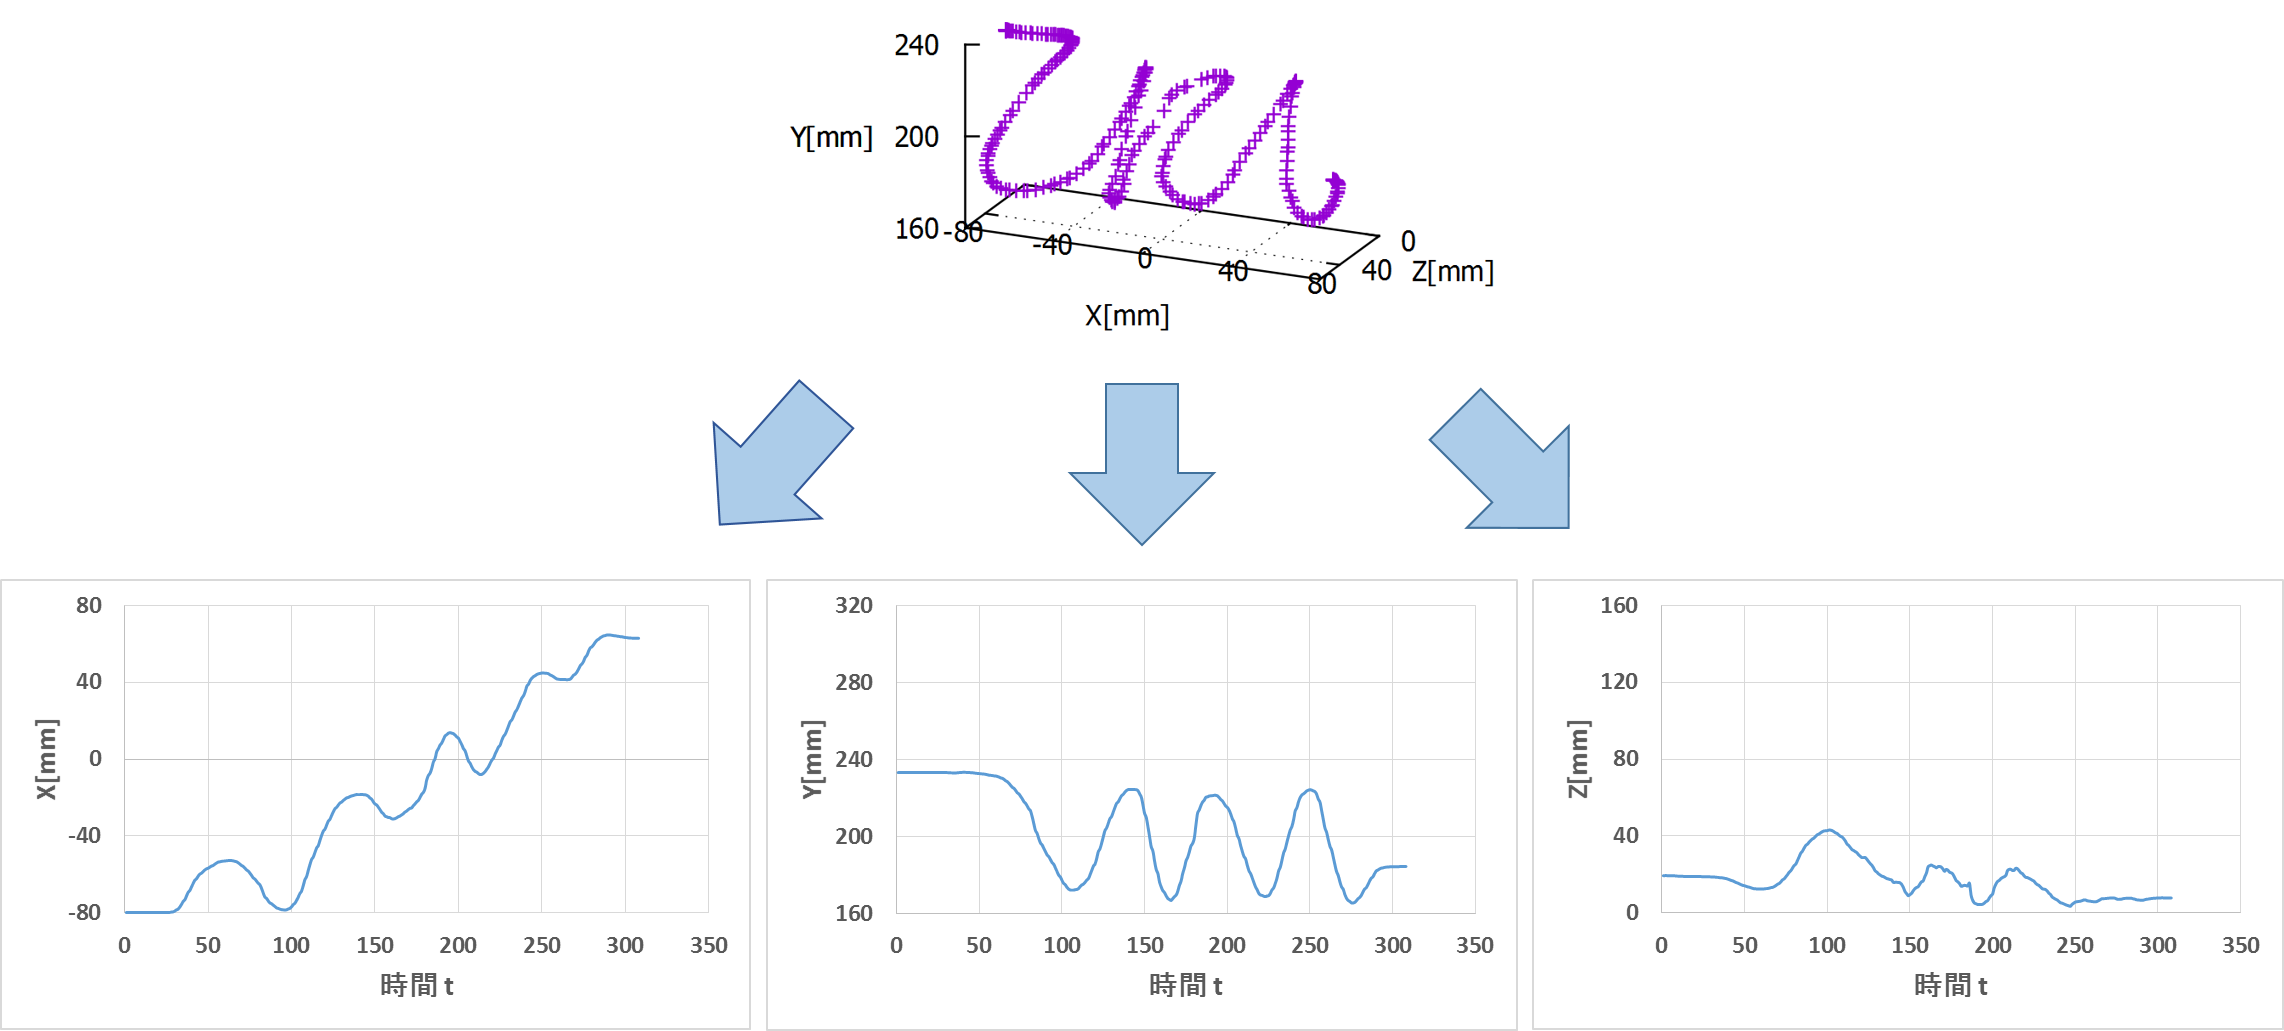
\includegraphics[clip,width=16.0cm]{./images/PreProcessing1.png}
    \caption{署名データをX軸, Y軸, Z軸の座標に分解}
    \label{fig:PreProcessing1}
  \end{center}
\end{figure}\\

\subsection{署名開始前・終了後の区間の削除}
各署名データには, 署名を書き始める前と書き終わった後の区間が含まれる. これらは座標データの始端・終端で座標の変化が殆ど無い部分
として現れる. データとしては意味のない区間であるため, 閾値処理によって削除する. 具体的には, XY平面において指先の初期座標から10mm以内の区間, または指先の最終座標から10mm以内の区間を署名開始前・終了後の区間として削除する. この時Z軸(奥行方向)を考慮しないのは, 署名時に意識的に指先を動かすのはX軸またはY軸方向についてであり, Z軸方向には意識的な動作は表れにくいと考えられるためである. 図\ref{fig:PreProcessing2}は図\ref{fig:PreProcessing1}に対し, 署名開始前・終了後の区間を削除したものである.
\\
\begin{figure}[htbp]
  \begin{center}
    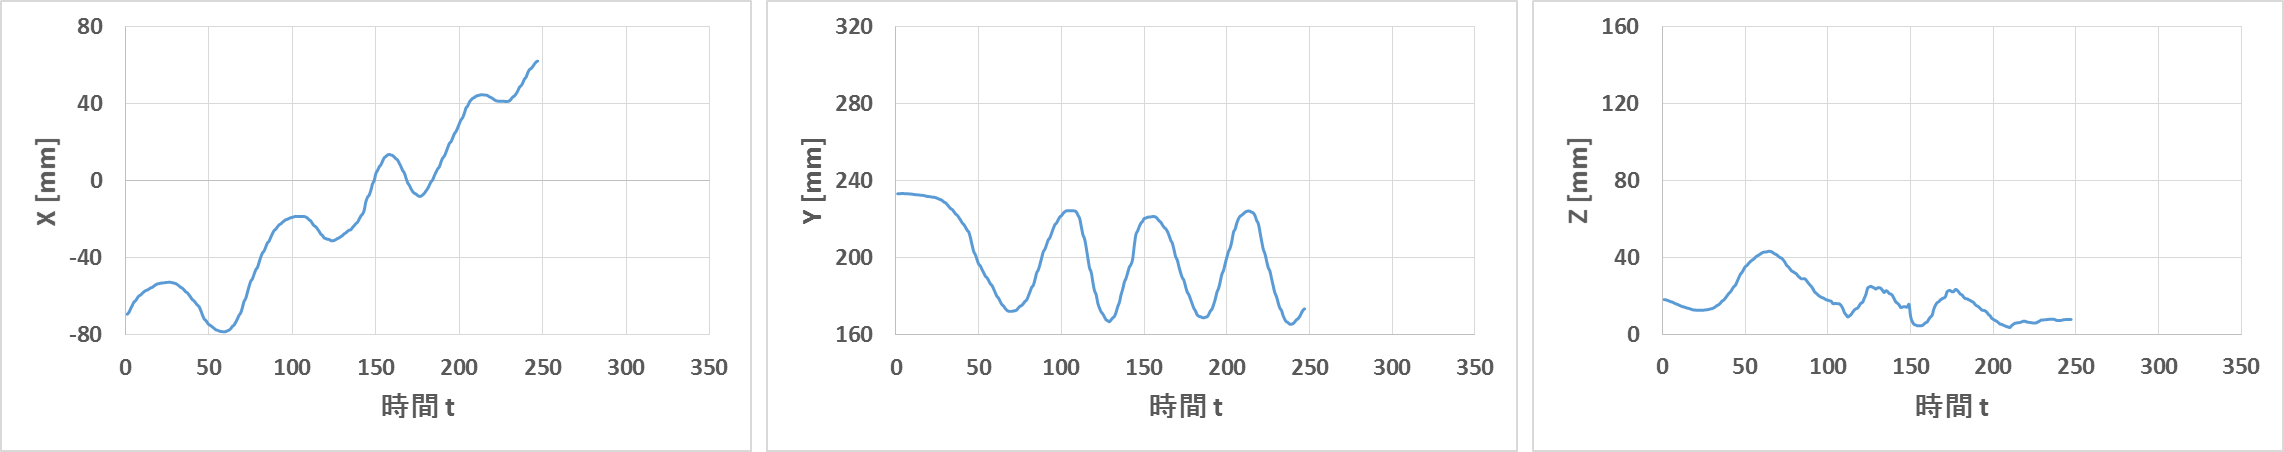
\includegraphics[clip,width=16.0cm]{./images/PreProcessing2.png}
    \caption{署名開始前・終了後の区間削除後}
    \label{fig:PreProcessing2}
  \end{center}
\end{figure}\\

\subsection{座標情報から動き情報への変換}

厳密な座標データは署名開始時点の座標の差により, 同一人物内においても大きく変化する. そこで, 座標データの時系列上で前後の点同士の差分を計算する. その際の計算式は

\begin{eqnarray}
x'_t & = & x_t - x_{t-1} \label{eq:eq1}
\end{eqnarray}
\\
となり, $x$はX軸の座標値, $t$は時間を示す. Y軸とZ軸についても同様に計算する. 直前の座標からの相対的な座標値とすることで署名毎の座標のずれを抑え, 各時間における指先の動き情報(どの軸の方向にどれだけ移動するか)に変換する. 図\ref{fig:PreProcessing3}は図\ref{fig:PreProcessing2}の座標情報から動き情報に変換したものである.
\\
\begin{figure}[htbp]
  \begin{center}
    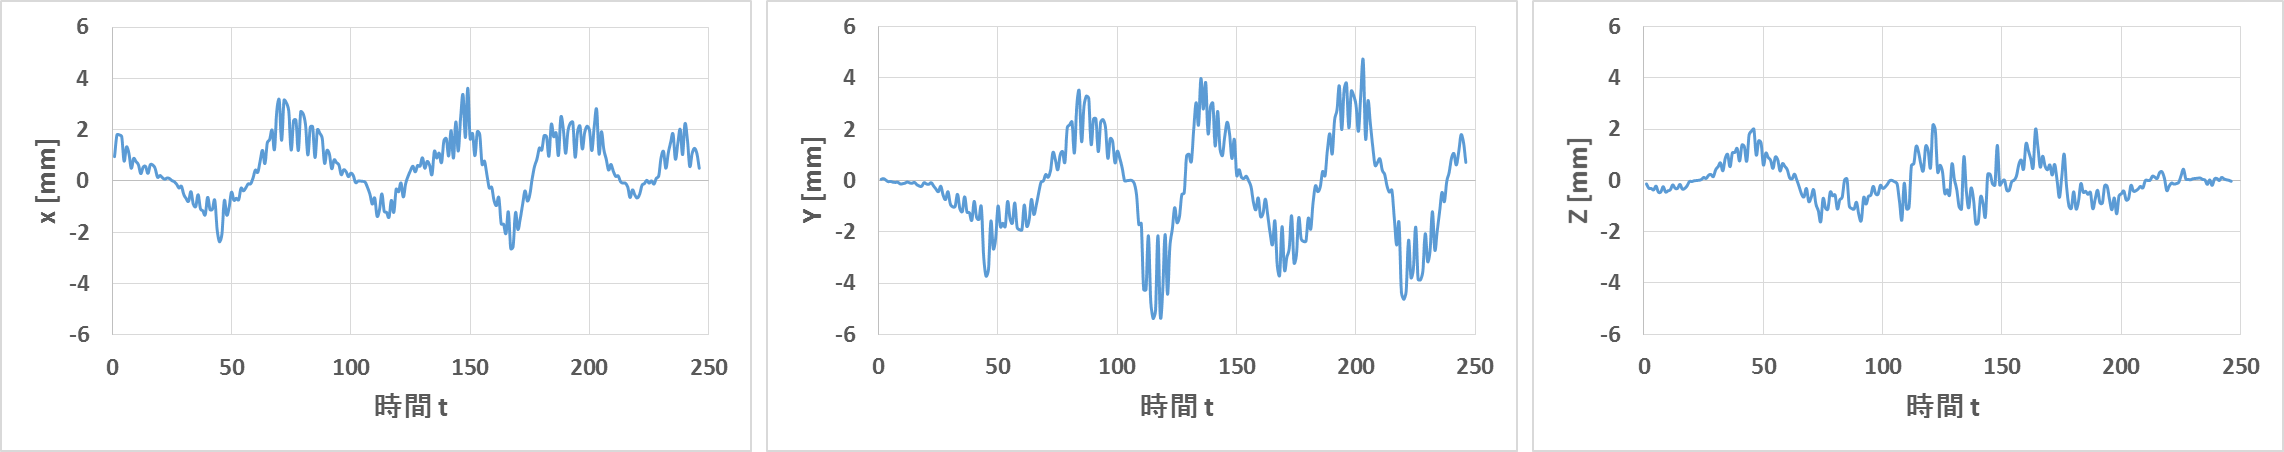
\includegraphics[clip,width=16.0cm]{./images/PreProcessing3.png}
    \caption{動き情報に変換後}
    \label{fig:PreProcessing3}
  \end{center}
\end{figure}\\

\subsection{データ長の統一}

通常, 計測された署名はデータ毎に長さ(時間)が異なる. しかし, 後述の畳み込みニューラルネットワークへ入力するためには全てのデータの長さを統一する必要がある. そこで本研究では線形補間法によりデータの長さを統一する. 
 
まず, 統一するデータの長さ$dst\_size$を決定し, 元データの長さ$data\_size$から必要な拡大・縮小倍率$scale$を求める.

\begin{equation}
scale = dst\_size / data\_size \label{eq:eq2}
\end{equation}\\

\noindent
次に, 補間後の点$t'$に対応する元データの点$t$を求める.

\begin{equation}
t = t' / scale \label{eq:eq3}
\end{equation}\\

\noindent
一般には図\ref{fig:PreProcessing4}のように, $t$は整数値とならず、元データの点同士の間に対応付けられる. ここで$\lfloor t \rfloor$は$t$を超えない最大の整数値である.

\begin{figure}[htbp]
  \begin{center}
    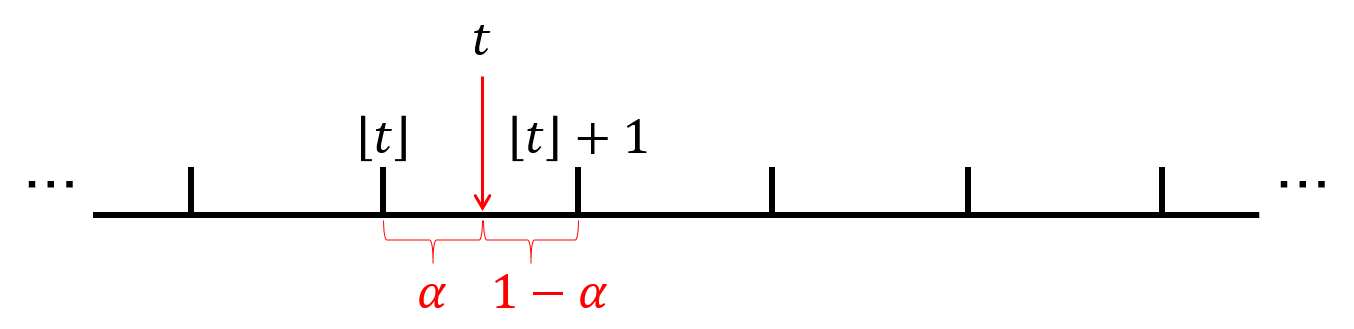
\includegraphics[clip,width=16.0cm]{./images/PreProcessing4.png}
    \caption{元データ上の対応点}
    \label{fig:PreProcessing4}
  \end{center}
\end{figure}

\noindent
ここで, 対応する点が存在しないため, $t$の前後の点の値(X軸であれば$x_{\lfloor t \rfloor}$と$x_{\lfloor t \rfloor + 1}$)を用いてデータを補完する. $t$と$\lfloor t \rfloor$の差を$\alpha$とし, 補間後の点の値を$x'_{t'}$とすると, 補間の式は

\begin{equation}
x'_{t'} = x_{\lfloor t \rfloor}(1 - \alpha) + x_{\lfloor t \rfloor + 1}\alpha \label{eq:eq4}
\end{equation}\\

\noindent
となる. Y軸とZ軸についても同様に計算する. 以上の処理を補間後のデータ内の点全てに対して行う. 図\ref{fig:PreProcessing5}は図\ref{fig:PreProcessing3}に対し, データ長を600として線形補間を適用した結果である.
\\
\begin{figure}[htbp]
  \begin{center}
    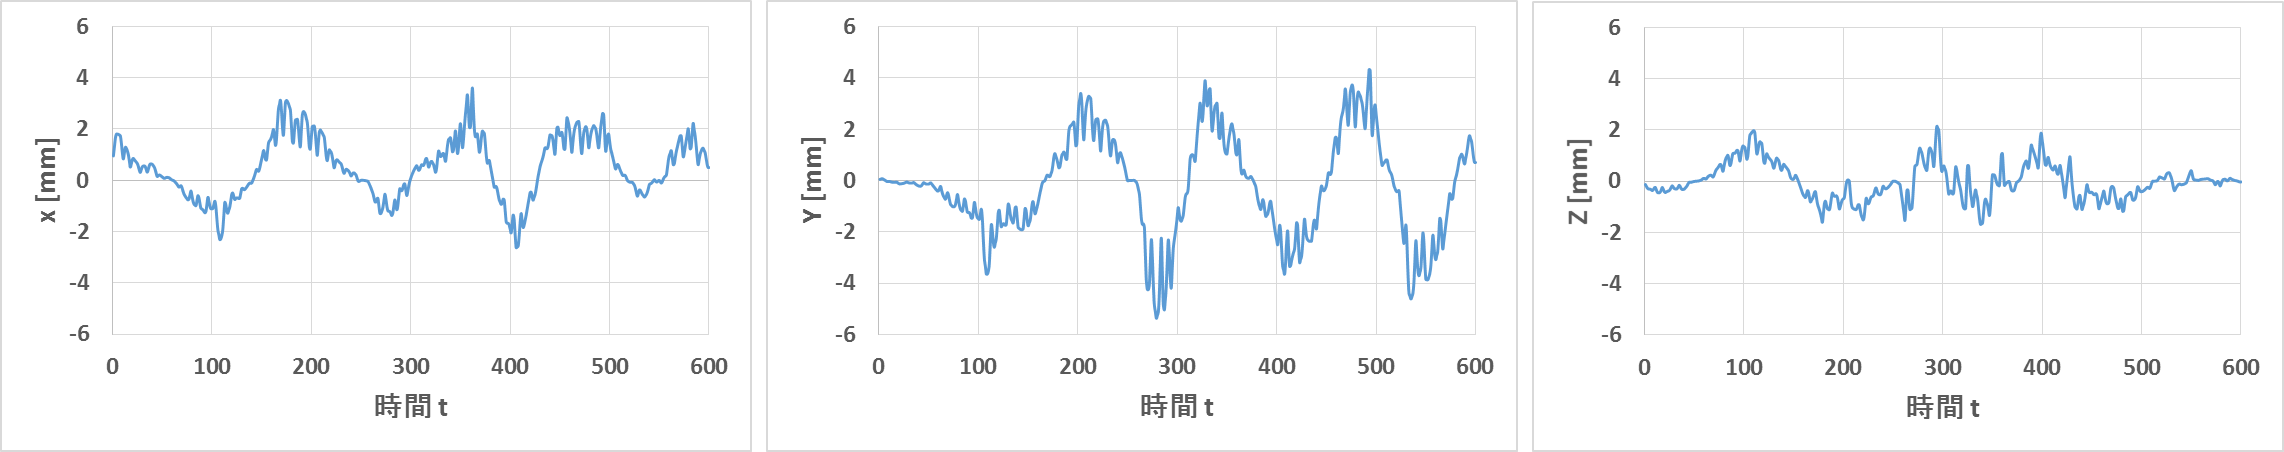
\includegraphics[clip,width=16.0cm]{./images/PreProcessing5.png}
    \caption{線形補間後のデータ}
    \label{fig:PreProcessing5}
  \end{center}
\end{figure}\\

\subsection{データ値のスケーリング}

署名開始前・終了後の区間の削除, 動き情報への変換, データ長の統一を行った後, データ値のスケーリングを行う. この処理は計測された全ての署名データを用いて行われる.

まず, データ間の偏りを失くすため, X軸, Y軸, Z軸それぞれについて全データにわたる平均値と標準偏差を計算する. そして全データから平均値を差し引き, 標準偏差で割ることで平均0分散1とする.

次に, 全データ中の値の範囲が$[-1.0:+1.0]$となるようにデータ値をスケーリングする. これは, 後述の畳み込みニューラルネットワーク内で扱う数値の範囲が$[-1.0:+1.0]$となっているためである. 時間$t$のデータの値$x_t$をスケーリングし$x'_t$を得るための計算式は

\begin{equation}
x'_t = \frac{x_t - x_{all\_min}}{x_{all\_max} - x_{all\_min}} \times 2 - 1 \label{eq:eq5}
\end{equation}\\

\noindent
となり, $x_{all\_max}$と$x_{all\_min}$はそれぞれ, 全データのX軸における最大値と最小値であり, Y軸とZ軸についても同様に計算する.
図\ref{fig:PreProcessing6}は図\ref{fig:PreProcessing5}に対してデータ値のスケーリングを行った結果である. 
\\
\begin{figure}[htbp]
  \begin{center}
    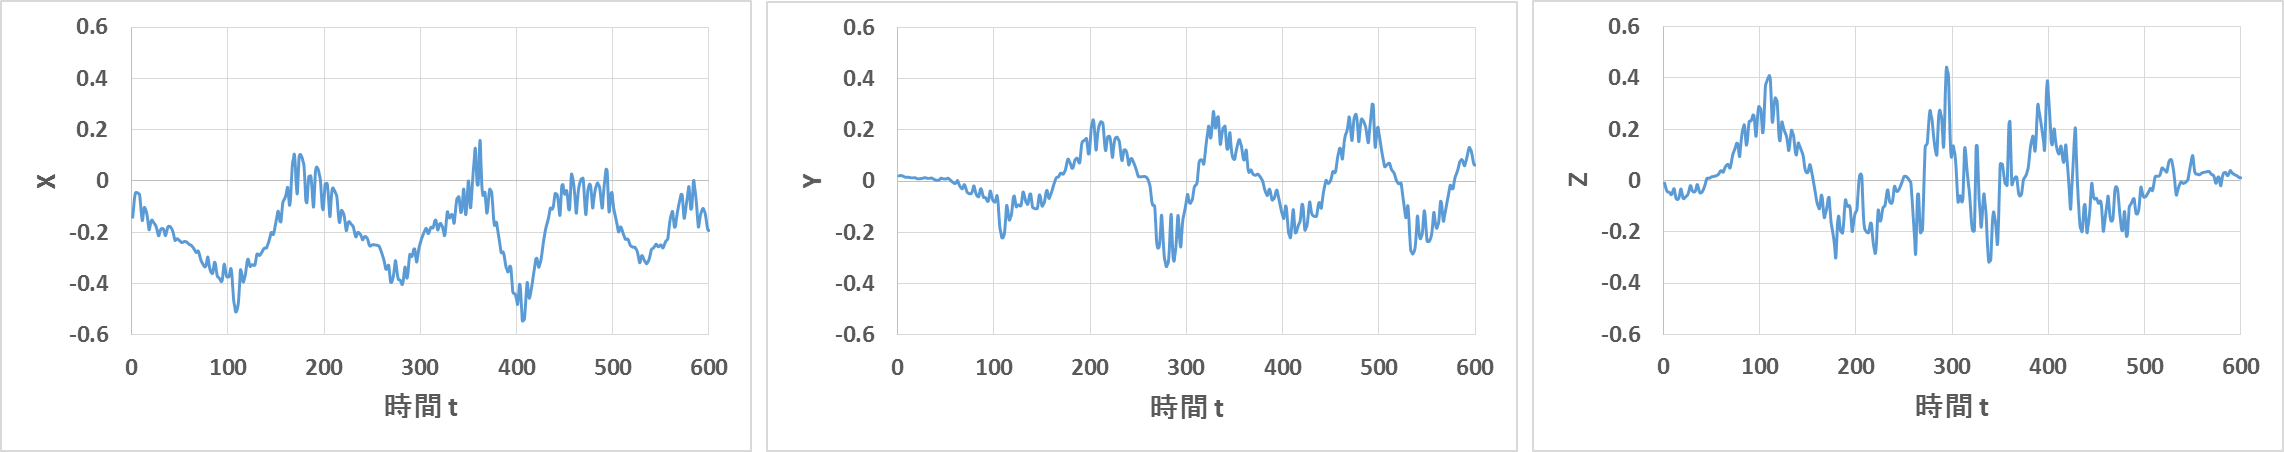
\includegraphics[clip,width=16.0cm]{./images/PreProcessing6.png}
    \caption{データ値のスケーリング後のデータ}
    \label{fig:PreProcessing6}
  \end{center}
\end{figure}\\

\subsection{学習用データの疑似生成}

本研究では, 畳み込みニューラルネットワークによる深層学習で署名データからの特徴抽出と識別を行う. 深層学習は機械学習手法の1つであり, 真筆と偽筆双方の学習用データが大量に必要となる. しかしながら本人による真筆とは異なり, 偽筆の学習用データについては大量に入手することが現実的に困難であると考えられる. よって, 少量の偽筆データを用意し, それらを元データとしてアフィン変換またはガウシアンノイズによる変形を加えることで必要な数の学習用偽筆データを疑似生成することとする. 以下でアフィン変換とガウシアンノイズについて説明する.\\

\subsubsection{アフィン変換}

アフィン変換は図形に拡大・縮小, 回転, 平行移動等の変換を行うための手法である. 3次元の図形に対する変換は以下のような$4\times4$行列を用いて表される.

\begin{equation}
  \begin{pmatrix} 
    x' &y' &z' &1
  \end{pmatrix} 
  =
  \begin{pmatrix} 
    x &y &z &1
  \end{pmatrix} 
  \begin{pmatrix} 
    a &b &c &0\\
    d &e &f &0\\
    g &h &i &0\\
    j &k &l &1
  \end{pmatrix} 
  \label{eq:eq6}
\end{equation}\\

\noindent
ここで, 式(\ref{eq:eq6})右辺の$a$, $b$, $c$, $d$, $e$, $f$, $g$, $h$, $i$, $j$, $k$, $l$を変更することで望む変換を実現可能であるが, 本研究においては拡大・縮小のみを適用することとする.回転については署名データを確認した結果, 回転を確認することができなかったため, 平行移動は前処理における動き情報への変換時に相殺されるため, 適用しない. 拡大・縮小を実現するためのアフィン変換の式は以下のようになる.

\begin{equation}
  \begin{pmatrix} 
    x' &y' &z' &1
  \end{pmatrix} 
  =
  \begin{pmatrix} 
    x &y &z &1
  \end{pmatrix} 
  \begin{pmatrix} 
    a &0 &0 &0\\
    0 &e &0 &0\\
    0 &0 &i &0\\
    0 &0 &0 &1
  \end{pmatrix} 
  \label{eq:eq7}
\end{equation}\\

\noindent
ここで, $a$, $e$, $i$はそれぞれ元データの座標値$x$, $y$, $z$に対する拡大・縮小倍率である.疑似生成された学習用偽筆データには他の署名データと同様に前述の前処理を順次適用する.\\

\subsubsection{ガウシアンノイズ}

ガウシアンノイズとは, 正規分布に従うノイズである. ノイズの平均を$\mu$, 分散を$\sigma^2$とすると, 正規分布は以下の確率密度関数を持つ.

\begin{equation}
p(x) = \frac{1}{\sqrt{2\pi\sigma^2}}exp\left(-\frac{(x-\mu)^2}{2\sigma^2}\right) \label{eq:eq8}
\end{equation}\\

\noindent
平均を0, 分散を1とした時の正規分布のグラフを図\ref{fig:GaussDist}に示す.
\\
\begin{figure}[htbp]
  \begin{center}
    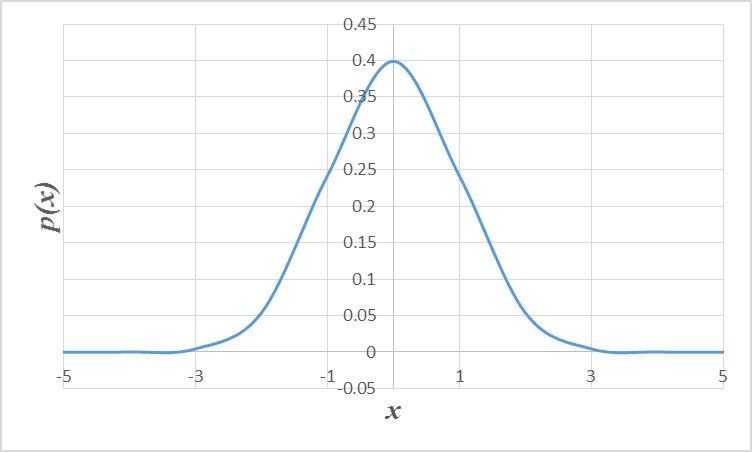
\includegraphics[clip,width=8.0cm]{./images/GaussDist.png}
    \caption{平均0分散1の正規分布}
    \label{fig:GaussDist}
  \end{center}
\end{figure}\\

\noindent
本研究では式(\ref{eq:eq8})の確率密度関数に従う乱数を生成し, 元データに加算する. ここで, 元となるデータは前述の前処理である“データ長の統一”を行った直後のデータであり以下の手順でノイズを加算した後, “データ値のスケーリング”を適用する. これは, 以下の手順中に全データの長さが等しくなければならないためである.\\
\begin{enumerate}
  \item 被験者Aに対する偽筆署名データ(元データ)を$N$個得る
  \item $N$個の元データ全てから時間$t = 0$における値を集め, X軸, Y軸, Z軸それぞれの分散$V_x(0)$, $V_y(0)$, $V_z(0)$を算出する. $t = 1, 2, ...$と同じ処理を繰り返し, 全ての時間$t$における分散$V_x(t)$, $V_y(t)$, $V_z(t)$を得る.
  \item 各元データの各時間について, 平均を0, 分散を2)で得た$V_x(t)$, $V_y(t)$, $V_z(t)$とした正規分布に従う乱数を生成し加算する.\\
\end{enumerate}

\noindent
複数のデータから分散を算出するため, 偽筆データのばらつきを考慮した疑似生成を行えると考えられる.

\newpage

\section{深層学習}

署名データからの特徴抽出・識別には深層学習\cite{cite_5}\cite{cite_6}を用いる. 深層学習とは多層ニューラルネットワークによる機械学習技術の総称である.その最大の特徴は特徴抽出と識別を同時に学習することであり,学習対象から識別に有効な特徴を自動的に見つけ出す.通常,物体認識等では手動での特徴設計を行い,試行錯誤を経て真に有効な特徴を決定する.しかし,深層学習ではネットワーク構造により多少の制限を受ける可能性はあるものの,特徴抽出と識別を一貫して学習するプロセスの中でより良い特徴を選択することが期待できる.そこで本研究では,画像のパターン認識等で実績のある畳み込みニューラルネットワークによる深層学習を行う.通常,時系列データを扱うニューラルネットワークとしてはリカレント型ニューラルネットワークの方が適している可能性がある.しかし本研究ではネットワークに入力するデータの差異による識別(クラス分類問題)を想定しているため,畳み込みニューラルネットワークを採用した. 以下にニューラルネットワークの基礎, 学習アルゴリズム, 本研究で使用する畳み込みニューラルネットワークについて述べる.\\

\subsection{ニューラルネットワーク}

\subsubsection{ニューラルネットワークの概要}

人間の神経系は, ニューロンとよばれる神経細胞が千数百億個集まって構成される. そして, ニューロンが巨大なネットワークを構築し神経伝達物質をやり取りすることで人間の高度な知的活動は行われている. 生物学におけるニューラルネットワークとは「神経回路網」のことであり, 人間を含む生体の神経系のネットワークのことである. 工学におけるニューラルネットワークは, この神経回路網を人工の素子を用いてコンピュータ上で再現し, 学習能力を付与することで様々な問題の解決を図ろうとするアプローチである. しかし, 工学上の手法としてモデル化されているため, 必ずしも神経系を忠実に再現したものではない.\\

\subsubsection{生体ニューロンの構造}

図\ref{fig:neuron}のように生体ニューロンは, 細胞体, 樹状突起, 軸索の3つの部位から成り立つ. 軸索はニューロン同士を結合し情報伝達を行う通信線であり, 先端は細かく枝分かれしている. そして他のニューロンの樹状突起または細胞体に結合し, その結合部をシナプスと呼ぶ. シナプスは完全に結合しているわけではなく, 実際には僅かな隙間がある. ニューロン間の情報伝達はこのシナプスを通じて神経伝達物質をやり取りすることで行われる.\\

\begin{figure}[htbp]
  \begin{center}
    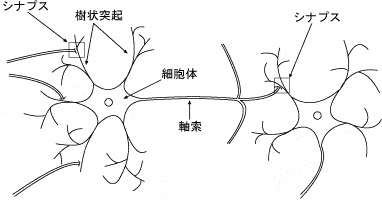
\includegraphics[clip,width=8.0cm]{./images/Neuron.png}
    \caption{生体ニューロン(注2)}
    \label{fig:neuron}
  \end{center}
\end{figure}

\subsubsection{生体ニューロンの情報伝達}

まず神経伝達物質は相手の細胞膜に作用し, 細胞内の電位を変化させる. そしてこの変化が一定のレベルに達すると細胞が興奮状態になり, 電位がインパルス状に立ち上がる. この時電位の変化が不十分な場合は何も起こらない. 発生したインパルスは軸索先端へと進み, 到達した時点で神経伝達物質が放出される. 以上がニューロン間の情報伝達の手順である. 巨大なネットワーク内で膨大な数のニューロンが情報伝達を行うことで生体は複雑な思考を行うことが可能となる.

\subsubsection{ニューロンモデルの構造}

工学におけるニューラルネットワークは図\ref{fig:neuron_model}のような, 生体ニューロンを模擬する人工の素子を用いて構成される.
実際の生体ニューロンの振る舞いは極めて複雑であるため単純な式で表すことはできない. よって人工の素子は, 特定の機能のみを抽出し単純化した工学的なモデルであり, 生体ニューロンを厳密に模倣したものではない.

\begin{figure}[htbp]
  \begin{center}
    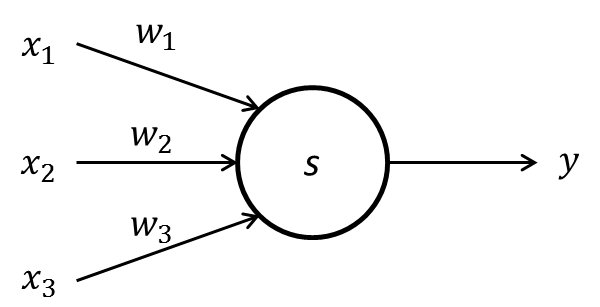
\includegraphics[clip,width=8.0cm]{./images/NeuronModel.png}
    \caption{ニューロンモデル}
    \label{fig:neuron_model}
  \end{center}
\end{figure}

\subsubsection{ニューロンモデルの情報伝達}
素子間の情報伝達方法としてはまず, いくつかの入力($x_1, x_2, \ldots $)が与えられる. そしてそれぞれの結合の重み($w_1, w_2, \ldots $)との積和が計算される. その結果, 設定された閾値$θ$を超えれば信号が出力される. 以上を式で表すと以下のようになる.

\begin{eqnarray}
  \displaystyle s &=& \sum_{n=1}^{N}w_nx_n
  \label{eq:neuron_model_1}\\
  \nonumber\\
  y &=& f(s-θ)
  \label{eq:neuron_model_2}
\end{eqnarray}

\noindent
ここで, $s$は素子への入力と重みとの積和である. $θ$は素子が持つ閾値であり, 常に1を出力する素子が$-θ$の重みで接続されていると考えれば, 閾値も重みの1つとして扱える. 関数$f$は活性化関数と呼ばれる. $s$と閾値$θ$の差に対して活性化関数$f$を作用させた値$y$ がそのまま素子の出力になる.ニューラルネットワークの活性化関数として用いられる関数には, シグモイド関数, ハイパボリックタンジェント関数などがある.\\

\begin{itemize}
  \item{シグモイド関数}\\
シグモイド関数は0.0から+1.0の連続的な値を出力する. $\alpha$はゲインと呼ばれ, この値が小さければグラフの傾きは緩やかになる.
逆に大きくなれば傾きは急になり, グラフの形はステップ関数に近くなる. 定義式とグラフは式(\ref{eq:sigmoid})と図ref{fig:sigmoid}のようになる.

\begin{equation}
  f(x) = \frac{1}{1+e^{-\alpha x}}
  \label{eq:sigmoid}
\end{equation}

\begin{figure}[htbp]
  \begin{center}
    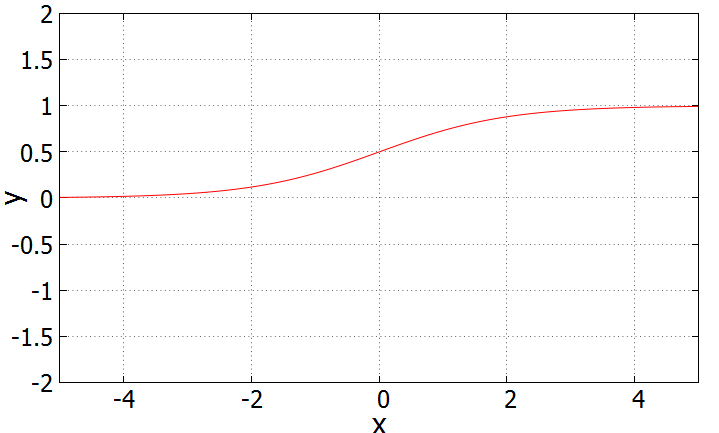
\includegraphics[clip, width=8.0cm]{./images/Sigmoid.png}
    \caption{シグモイド関数}
    \label{fig:sigmoid}
  \end{center}
\end{figure}

  \item{ハイパボリックタンジェント関数}\\
ハイパボリックタンジェント関数は-1.0から+1.0の間で連続的な値を出力する. 定義式とグラフは式(\ref{eq:tanh})と図\ref{fig:tanh}のようになる.

\begin{equation}
  f(x) = \frac{e^x-e^{-x}}{e^x+e^{-x}}
  \label{eq:tanh}
\end{equation}

\begin{figure}[htbp]
  \begin{center}
    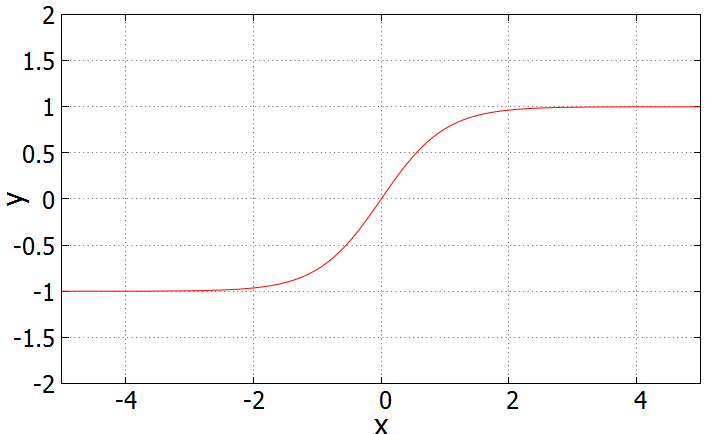
\includegraphics[clip, width=8.0cm]{./images/tanh.png}
    \caption{ハイパボリックタンジェント関数}
    \label{fig:tanh}
  \end{center}
\end{figure}
\end{itemize}

\subsubsection{ニューラルネットワークのネットワークモデル}

ニューラルネットワークの工学的モデルは上述の素子(以下ユニット)を多数接続させて構成されている.また, 図\ref{fig:network_model}のように階層構造になっている.

\begin{figure}[htbp]
  \begin{center}
    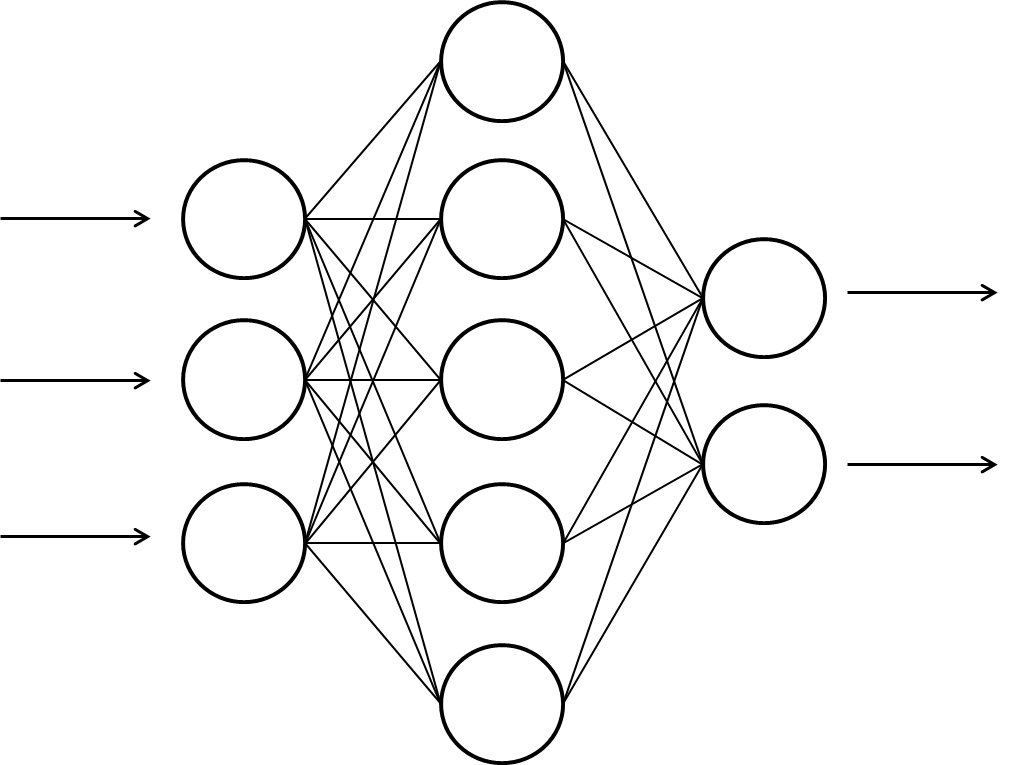
\includegraphics[clip,width=8.0cm]{./images/NetworkModel.png}
    \caption{ネットワークモデル}
    \label{fig:network_model}
  \end{center}
\end{figure}

図\ref{fig:network_model}は 3 層構造となっており, 左から入力層・中間層・出力層となっている. 入力層にはネットワークへの入力が与えられ, 出力層はネットワークの出力を行う.中間層はこれら 2 つの層の間に位置し, 与えられた入力を変換し出力層へ伝える. 複数の中間層が設置されることもあり, 最適なネットワーク構造は扱う問題によって異なる. また図\ref{fig:network_model}は入力側から出力側へ 1 方向のみに信号が伝わるフィードフォワード型ニューラルネットワークであり, この方法では, ネットワークに入力を与えると出力側へ向けて素子の出力値は次々に決まっていく.

\newpage
\subsection{誤差逆伝播法}

誤差逆伝播法は教師あり学習のアルゴリズムの1つである. 目標とする入出力関係を表す関数を近似するように重み及び閾値を勾配法に基づいて修正する. 勾配法とは, 問題を適当な評価関数の最小化として定式化し, 評価関数の勾配 (偏微分) を用いてパラメータの微小修正を繰り返す非線形関数の近似手法である. ニューラルネットワークにおけるパラメータとは重みと閾値である. 評価関数にはクラス分類問題であれば交差エントロピー誤差がよく用いられる.

誤差逆伝播法の具体的な手順としてはまず, 学習用サンプルが1つ与えられ各ユニットの出力が計算される. 第$l$層($1 \leq l \leq L $)のユニット$j (1 \leq j \leq J)$の出力計算は式(\ref{eq:neuron_model_1})(\ref{eq:neuron_model_2})を元にして次のように表すことが出来る.

\begin{eqnarray}
  \displaystyle s_{j}^{(l)} &=& \sum_{i=1}^{I}w_{ji}^{(l)}y_{i}^{(l-1)}\\
  \nonumber \\
  y_{j}^{(l)} &=& f(s_{j}^{(l)})
  \label{eq:bp_1}
\end{eqnarray}

\noindent
ここで$I$は第$(l-1)$層の素子数である. $w$は閾値を含む重みで$y$は素子の出力値である. この計算を出力層まで繰り返し行うことでネットワークの出力が得られる. そして得られた出力と与えられた学習用サンプルに対応する教師信号$t$を用いて評価関数を計算し, 出力の誤差$E$を得る. 評価関数として交差エントロピー誤差を用いた場合の計算式は

\begin{equation}
\displaystyle E = -\frac{1}{N}\sum_{n=1}^{N}\sum_{j=1}^{J}\left(t_{j}log(y_{j}^{(L)}) + (1 - t_{j})log(1 - y_{j}^{(L)})\right)
\end{equation}

\noindent
となる. ここで$N$は学習サンプルの数である.






























